%%
%% 研究報告用スイッチ
%% [techrep]
%%
%% 欧文表記無しのスイッチ(etitle,eabstractは任意)
%% [noauthor]
%%

\documentclass[submit,techrep]{ipsj}
% \documentclass[submit,techrep,noauthor]{ipsj}



\usepackage[dvips]{graphicx}
\usepackage{latexsym}
\usepackage{cite}


\def\Underline{\setbox0\hbox\bgroup\let\\\endUnderline}
\def\endUnderline{\vphantom{y}\egroup\smash{\underline{\box0}}\\}
\def\|{\verb|}
%

%\setcounter{巻数}{59}%vol59=2018
%\setcounter{号数}{10}
%\setcounter{page}{1}


\begin{document}


\title{狭小空間監視のためのドローンを利用した\\ AR可視化手法の実装と評価}

\etitle{Implementation and Evaluation of a Drone-Based\\ AR Visualization Method for Narrow Space Surveillance}

\affiliate{doshisha}{同志社大学大学院 理工学研究科\\Graduate School of Science and Engineering, Doshisha University}

\affiliate{mobility}{同志社大学モビリティ研究センター\\Mobility Research Center, Doshisha University}


\author{竹内 一真}{Kazuma Takeuchi}{doshisha}[kazuma.takeuchi@nislab.doshisha.ac.jp]
\author{滕 睿}{Rui Teng}{mobility}
\author{佐藤 健哉}{Kenya Sato}{doshisha}


% --------------------------- Abstract  ---------------------------

\begin{abstract}

近年,小型ドローンは機体が小さいことから,人間が入れないような狭小空間での活躍が期待されている.しかし,狭小空間では遮蔽物が多いため,操縦者の死角領域内にてドローンを飛行させる必要があり,操縦は困難である.また小型ドローンは,センサ搭載制限があり,センサによる障害物回避を行うことが困難であるため,衝突する恐れのある障害物が多く存在する狭小空間では,安全なドローン操縦は困難である.そこで,操縦者とドローンの間に遮蔽物が存在し,ドローンを視認できない環境に対してARを用いる.本稿では,三次元環境地図を事前に作成し,遮蔽物により視認できない空間,ドローンを可視化した上で,ARを用いたドローン近傍の障害物を知覚する方式を提案し,従来の操縦とARを用いた方式を比較した評価した.その結果,ARありの方式では一貫して平均操縦時間,平均衝突警告回数が減少し,操縦性の向上を示した.

\end{abstract}

\begin{jkeyword}
拡張現実,無人航空機,点検,三次元環境認識,可視化
\end{jkeyword}

\begin{eabstract}

In recent years, small drones have been expected to play an active role in narrow spaces where humans cannot enter due to the small size of the spaces. However, since there are many obstructions in a small space, it is necessary to fly the drone within the pilot's blind spot, which is difficult to control. In addition, small drones are limited in sensor installation, and it is difficult to avoid obstacles using sensors, making safe drone operation difficult in confined spaces with many obstacles that may cause collisions. Therefore, AR is used for the environments where the drone cannot be seen due to the presence of obstructions between the operator and the drone. In this paper, we propose a method of perceiving obstacles in the vicinity of a drone using AR on the basis of creating a three-dimensional map of the environment in advance and visualizing the space and drone that cannot be seen due to obstructions. As a result, the average maneuvering time and the average number of collision warnings were consistently reduced in the method with AR, indicating an improvement in maneuverability.

\end{eabstract}

\begin{ekeyword}
Augmented reality, unmanned aerial vehicle, inspection, 3D environment recognition, visualization
\end{ekeyword}

\maketitle

% --------------------------- Section1  ---------------------------
\section{はじめに}

近年,多方面でのドローンを活用した事業が進出しており,インフラ点検や災害調査など,応用分野を拡大しながら,世界のドローン市場は急速に成長している\cite{Nonami}.中でも小型ドローンの特徴である機体の大きさを活かして,人間が入れないような狭い空間での活躍の場も増加している.しかし,狭小空間でのドローン飛行は,遮蔽物が多く,操縦者は遮られた視点からの操縦を必要とする.そのため,死角領域内のドローン操縦では,ドローンを視認できない中,衝突することなく,安全に操縦する技術が求められる.
\par
オンボードカメラ搭載ドローンを使用する場合では,操縦者は,ドローンから送られる空撮した映像を元に操縦が可能となる.このようなドローン操縦方法では,実際の現実空間を映像として見ながら操縦できるため,現実のドローンを視認することなく,狭小空間を探索することができる.しかし,カメラが前方しか写さないことにより,前方以外の死角が多くなり,状況認識が不十分となるため\cite{Green},狭小空間のように狭く,障害物が多いような環境では,操縦は困難である.
\par
操縦者視点でドローンを視認し飛行させる三人称視点操縦の場合では,ドローン中心の一人称視点での操縦に比べて,ドローン周辺の状況を把握することができ,また,ドローンの実際の高さや位置を正確に把握することができる\cite{Green}.しかし,三人称視点操縦では,操縦者から見えるドローンまでの距離感が掴めないため\cite{Zollmann},ドローン周辺の障害物へ衝突する恐れがある.
大型ドローンでは,自律飛行や障害物回避などの機能が実現されているが,センサ搭載制限のある小型ドローンでは,障害物回避の支援がないことが多く,衝突の危険性がある.また,障害物回避を搭載していても,狭小空間では障害物回避が行えない場面が多く存在する\cite{syohou}.
\par
本研究では,狭小空間による死角領域内のドローン飛行の危険性を軽減するため,Augmented Reality(AR)により操縦者の死角領域内を可視化した三人称視点によるドローン操縦を実現する.また,狭小空間における障害物回避に有効な情報を確かめるため,ドローン近傍の障害物を検知するAR方式を提案する.

% --------------------------- Figure  ---------------------------

\begin{figure}[tb]
\centering
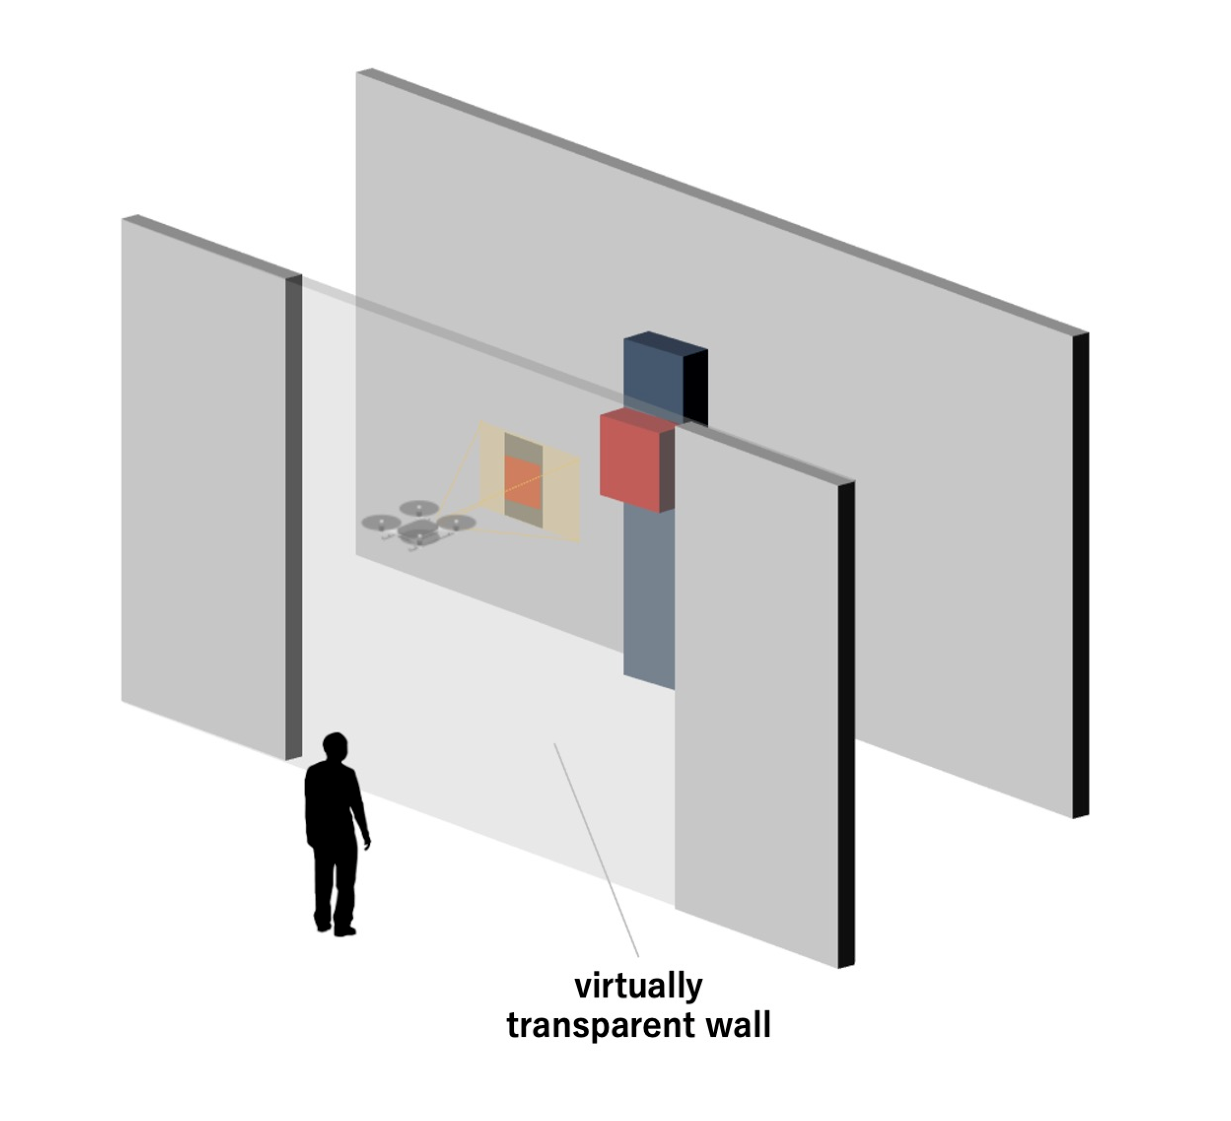
\includegraphics[width=\linewidth]{img/02_relation.eps}
\caption{死角領域内のAR可視化}
\ecaption{AR Visualization in the Blind Spot Area}
\label{fig:02_relation}
\end{figure}

% -----------------------------------------------------------------

% --------------------------- Section2  ---------------------------
\section{関連研究}
\subsection{狭小空間探索にARを適用することの有意性}
Walkerらの研究\cite{Walker}では,ARが人間とドローンの相互作用をどのように媒介するかを調査することで,ドローンの意図を視覚的に伝えるための一連の明示的・暗示的なデザインを開発し,ユーザ研究で評価を行った.
その結果,ドローンに対しARを用いたデザインは,ARなしと比べ,課されたタスク効率を大幅に向上させ,ARを用いることでドローンの操縦性を向上させるための,直感的で視覚的な合図を提供することが可能であることが示された.

Hedayatiらの研究\cite{Hedayati}では,オンボードカメラ搭載ドローンの空撮した映像を,AR可視化する手法を提案している.結果として,遠隔操作におけるドローン飛行の衝突回数を減少させた.

Kamedaらの研究\cite{Kameda}では,監視カメラが埋め込まれた場面において,カメラ付きhandy subnotebook PC(HPC)を用いた新しい屋外型複合現実感システムを提案しており,建物や壁などの構造物に隠れて見えない不可視領域の状況を,リアルタイムで可視化できることを示した.

このように,ドローンや死角領域に対してARを用いた前例があり,狭小空間による死角領域内のドローン飛行においても適合すると推測する.

%2.2
\subsection{狭小空間におけるドローン操縦手法}

Liuらの研究\cite{Liu}では,ドローン周辺の環境を再構築し,操縦者前方の床やテーブル上に3Dマップを表示することにより,自律航行中のドローンとの直感的なインタラクション手法を提案している.
結果として,操縦者はドローン周辺の三次元環境に没入することができ,飛行空間の探索に成功することができた.
しかし,自律飛行することのできない狭小空間では,操縦者の意図を伝えて飛行させることができない.また,デスクトップPCインタフェースと比較評価した結果,ARインタフェースは操作精度を犠牲にしていた.そのため,タスク完了までに時間がかかる問題を抱えており,ドローン操縦性を低減してしまう.

Eratらの研究\cite{Erat}では,狭小空間による死角領域内の,三人称視点ドローン操縦手法を提案している.図\ref{fig:02_relation}が示すように,事前に空間マッピングにて用意した三次元環境を用いて,閉鎖環境をAR可視化している.
結果として,三人称視点ドローン操縦手法では,タスク完了までの操縦時間が半分以下となった.

しかし,ドローン飛行の際に,障害物に衝突しない環境を想定しており,狭小空間での障害物による危険性が提示されていない.また,一人称視点操縦では,ジョイパッドを用いて操縦していた一方で,三人称視点操縦では,ハンドジェスチャで操縦していた.そのため,タスク完了までの操縦時間への有意差が,ARによる空間認識の提供により引き起こされたか不明である.そのため,ARにより狭小空間でのドローン操縦性向上が示せるかを確認するため,衝突の危険性を提示し,また,ドローン操縦法を統一する必要がある.

% --------------------------- Figure  ---------------------------

\begin{figure}[tb]
\centering
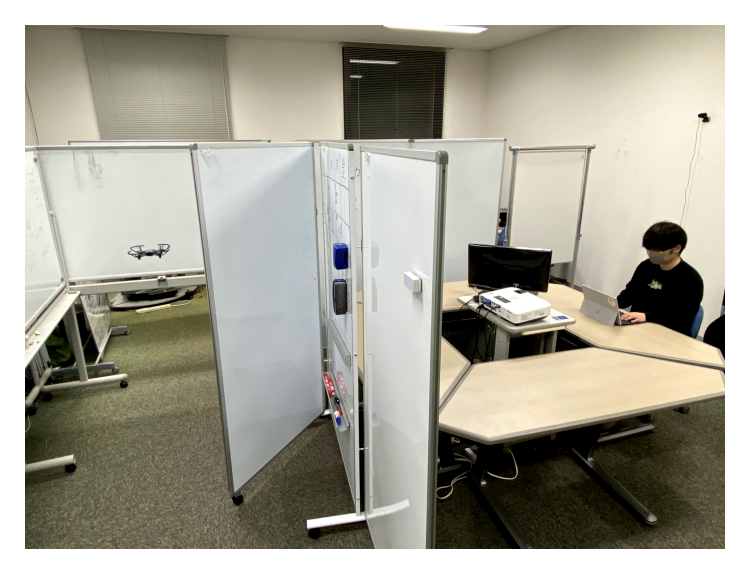
\includegraphics[width=\linewidth]{img/03_enviroment.eps}
\caption{死角領域内におけるドローン操縦環境}
\ecaption{Drone Control Environment in the Blind Spot Area}
\label{fig:03_enviroment}
\end{figure}

\begin{figure}[tb]
  \centering
  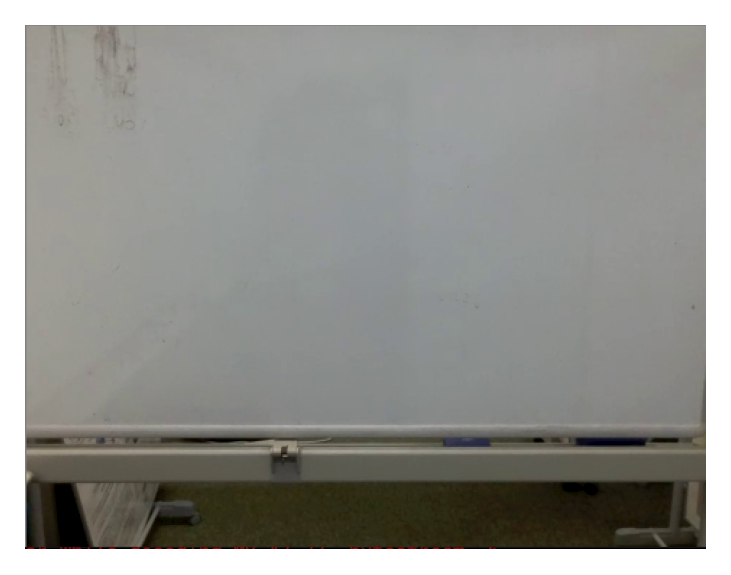
\includegraphics[width=\linewidth]{img/03_fpv.eps}
  \caption{一人称視点方式による操縦画面}
  \ecaption{First-Person View Control Screen.}
  \label{fig:03_FPV}
\end{figure}

\begin{figure}[tb]
\centering
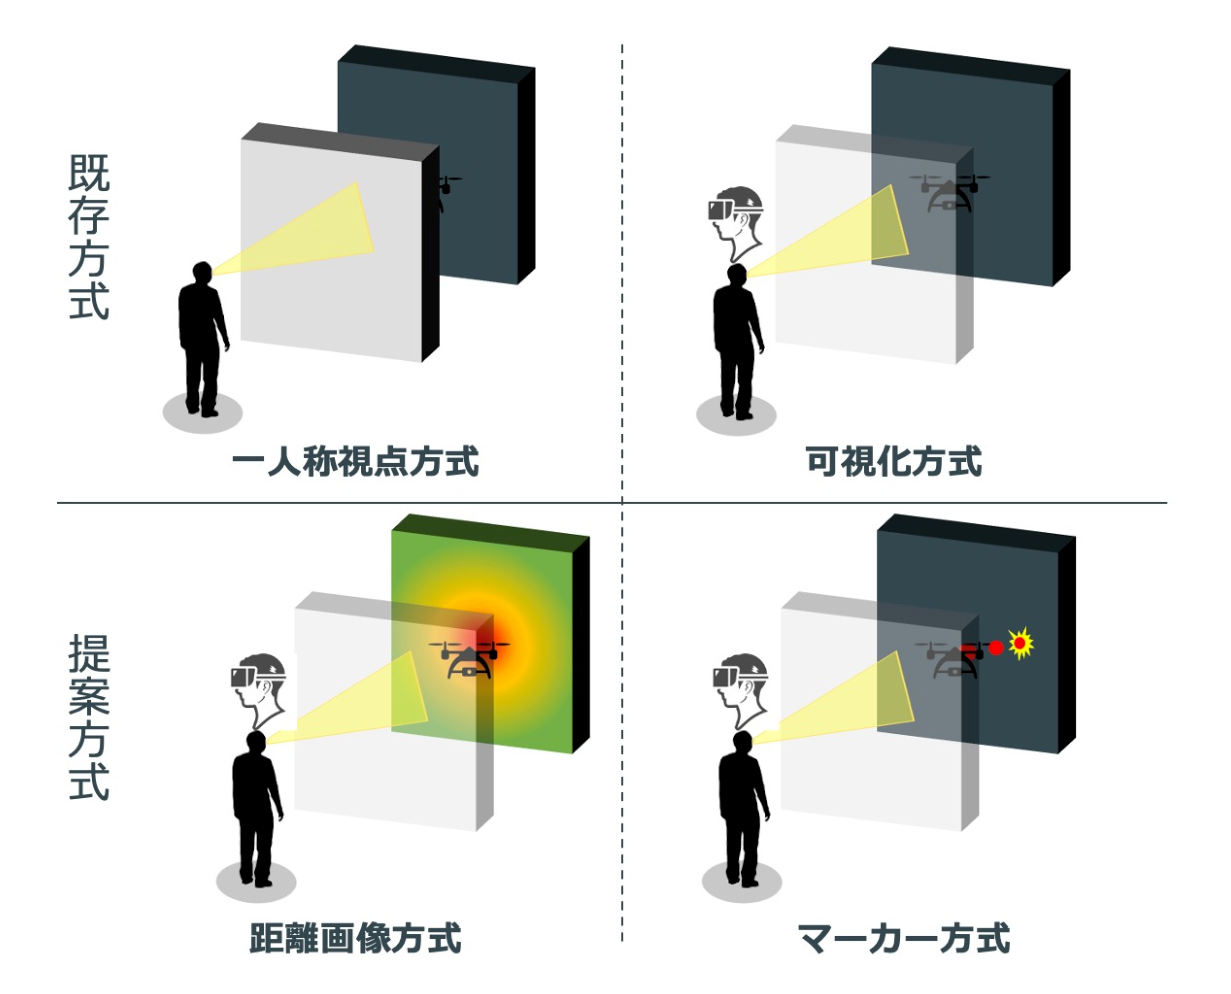
\includegraphics[width=\linewidth]{img/03_outline.eps}
\caption{提案方式概要}
\ecaption{Outline of Proposed Method}
\label{fig:03_outline}
\end{figure}

\begin{figure*}[!tb]
  \centering
  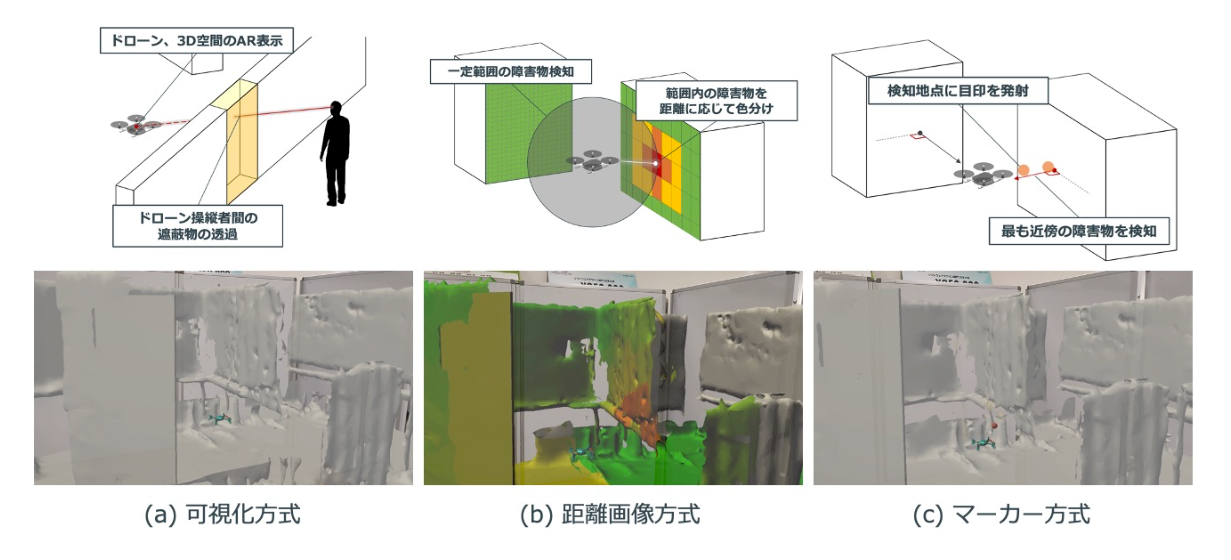
\includegraphics[width=\linewidth]{img/03_preview.eps}
  \caption{各方式の概要および操縦者目線}
  \ecaption{Overview of Each Method and the Pilot's Perspective}
  \label{fig:03_preview}
\end{figure*}

% -----------------------------------------------------------------

% --------------------------- Section3  ---------------------------

\section{提案方式}
\subsection{概要}
本研究では,狭小空間により,操縦者と小型ドローン(以下,ドローン)の間に遮蔽物があり,ドローンを視認できない環境を「死角領域」とする.図\ref{fig:03_enviroment}の環境におけるドローン操縦を想定しており,ARを用いて死角領域内の空間認識を提供し,ドローン周辺の障害物を知覚させることで,ドローン操縦性を向上させる.
\par
先に述べた先行研究\cite{Erat}を元に,2つのドローン操縦方式を用意し,一人称視点方式,可視化方式と呼ぶことにする.
図\ref{fig:03_FPV}に示しているようなドローンの空撮した映像を頼りに操縦を行う,従来のドローン操縦手法である一人称視点方式と,\ref{fig:02_relation}を参考に作成した,ARを用いて死角領域内の空間認識を提供する可視化方式を比較することにより,先行研究の問題点である,死角領域内へのAR適用の有用性を検討する.
また,本研究では可視化方式を元に,ドローン周辺の障害物知覚を支援する2つの方式を提案する.
この2つの方式を,距離画像方式,マーカー方式と呼ぶことにする.
4つの方式を比較することで,どのような情報が死角領域内のドローン操縦に有効であり,操縦性の向上を示せるか評価した.
各方式の概要を図\ref{fig:03_outline}に示す.以降の節では一人称視点方式,可視化方式,距離画像方式,マーカー方式の4つの方式の詳細について説明する.


\subsection{一人称視点方式}
一人称視点方式では,操縦者はドローンから送られる空撮した映像を基に,ドローン中心の一人称視点での操縦を行う.
本研究では死角領域内での操縦を前提としているため,操縦者はドローンから送られる空撮した映像のみを頼りに操縦を行う.
\par
図\ref{fig:03_FPV}は,ドローンから送られている空撮した映像を示しており,操縦者はこの映像をもとにドローン操縦を行う.


\subsection{可視化方式}
可視化方式では,ドローンと操縦者の間に遮蔽物が存在すると判断した際,ドローンが飛行している場所を操縦者にとっての死角領域とし,事前に空間マッピングした三次元環境地図における遮蔽物を透過した上で,現実環境に重畳表示することで,死角領域の空間認識を提供する.操縦者は,死角領域内を飛行するドローンを視認することはできないが,ARによって仮想のドローンと,ドローン周辺の三次元環境を視認することができる.
\par
図\ref{fig:03_preview}左のように,遮蔽物によって視認できないドローンと,そのドローン周辺の環境をARによって可視化している.障害物を知覚せず,可視化による空間認識の視覚支援のみを行なっている.


\subsection{距離画像方式}
距離画像方式は,ステレオビジョンを参考にして,ドローンから障害物までの距離に応じて,障害物の色を分けている.障害物を3色に分類することで,近傍の障害物の危険性を警告する.
距離画像方式は,全体的な環境の理解を提供しており,ドローン周辺の障害物に対する衝突の危険性を示す.
\par
距離画像方式では,障害物までの危険な距離を閾値a,未だ猶予はあるが慎重に動くべき距離を閾値bとする.
常に周りの障害物までの距離を計測し,閾値を元に以下のいずれかの動作をする.

\begin{enumerate}
	\item ドローンからの距離が閾値a 以内の障害物を赤色に変更
    
    \item ドローンからの距離が閾値a 以降 〜 閾値b 以内の障害物を赤色から黄色に変更
    
    \item ドローンからの距離が閾値b 以降の障害物を緑色に変更
\end{enumerate}

図\ref{fig:03_preview}中央のように,ドローン本体ではなく,ドローン周辺の環境を拡張しており,ドローン周辺の障害物の危険度を理解できる,色彩による視覚支援を行なっている.赤色に変化した障害物の方向には衝突の危険性,黄色になっている障害物の方向には慎重な操縦の必要性,一方で緑色の障害物の方向には進んでも衝突の危険性がないことを示し,操縦者への安心感を提供する障害物知覚を行っている.



\subsection{マーカー方式}
マーカー方式は,ドローンから見て最も近い障害物に対して,障害物までの距離に応じて,色分けを行なった目印を付けている.距離画像方式では障害物すべてが色分けされているため,操縦者を混乱させる可能性がある.マーカー方式では,選択的注意を参考に,最も危険な障害物のみを知覚させるため,距離画像方式に比べ簡易的なアプローチとなっている.
\par
マーカー方式では,障害物までの危険な距離を閾値a,未だ猶予はあるが慎重に動くべき距離を閾値bとする.
常に周りの障害物までの距離を計測し,閾値を元に以下のいずれかの動作をする.

\begin{enumerate}
	\item ドローンからの距離が閾値a 以内の最も近傍の障害物に対して赤色の目印を示す
    
    \item ドローンからの距離が閾値a 以降 〜 閾値b 以内の最も近傍の障害物に対して黄色の目印を示す
\end{enumerate}

図\ref{fig:03_preview}右のように,ドローン自体を拡張しており,どの障害物が危険か一目で理解できる,直感的視覚支援を行なっている.赤色の目印が向けられている障害物はこれ以上進むと衝突の危険性があり,黄色の目印が向けられている障害物は慎重な操縦を求め,操縦者への危機感を与える視覚的支援を行なっている.

% --------------------------- Section4  ---------------------------

\section{評価}

\subsection{実装環境}
システム構成を図\ref{fig:04_system}に示す.
実際に使用したドローンはRyze Tech社製Tello EDU(以下,Tello)であり,操作端末はMacBookProを用いる.Telloはプログラミングによってフライトコントロールを行うことができ,規定のコマンドを送信することで飛行制御することができる.
\par
ARHMDはMicrosoft HoloLens2(以下,HoloLens)を使用する.
事前に,HoloLensのSpatial Mappingにより空間マッピングを行うことで空間のメッシュデータを入手し,静的な三次元環境地図を作成する.
作成した三次元環境地図を,ゲーム・アニメーションエンジンであるUnity内の3D仮想空間上に配置し,操縦者の位置情報と,Unity内の三次元環境地図の位置合わせを行うことで,空間認識を提供する.
\par
サーバではTello,HoloLensとUDP通信を行なっており,常時,Telloの傾きや移動距離をHoloLensに送信することで,3D仮想空間上に存在するドローンとの位置合わせを行っている.ここでUDPを使用する理由として,Tello,サーバ,HoloLens間の遅延低減を目的とする.
\par
距離画像方式,マーカー方式では,共に障害物までの距離によって,危険度を色で示している.操縦者がドローンを操縦するとき,衝突する危険性がある距離を0.3mとし\cite{Yamada},距離画像方式では,障害物までの距離が0.3mまでを赤色,0.3m〜0.6mまでを黄色,0.6m以上を緑色で示す.マーカー方式では障害物までの距離が0.3mまでを赤色の目印,0.3m〜0.6mの際に黄色の目印を示す.


% --------------------------- Figure  ---------------------------

\begin{figure}[tb]
\centering
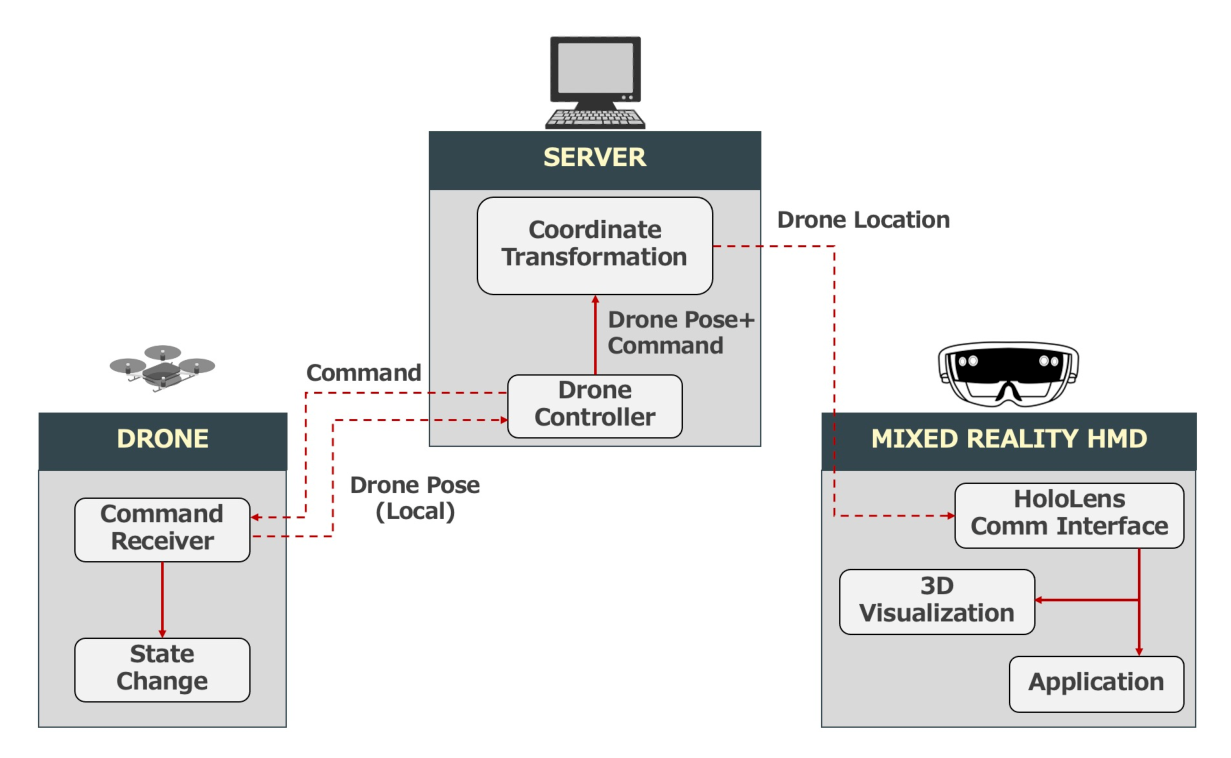
\includegraphics[width=\linewidth]{img/04_system.eps}
\caption{システム構成}
\ecaption{System Configuration}
\label{fig:04_system}
\end{figure}

% -----------------------------------------------------------------

\subsection{タスク}
実験環境は図\ref{fig:04_experiment}に示すように,スタート地点,障害物,ゴール地点で構成されており,実験参加者は,ドローンをスタート地点から目的地まで操縦し,目的地で着陸するタスクを行った.その間,上下左右に移動しなければ衝突の恐れがある障害物を設置した.図\ref{fig:04_experiment}に赤色で示されている障害物を回避する必要があり,避けなければ通過が困難になるよう設定している.実際の狭小空間では,速さではなく,衝突のない安全飛行が必要であるため,参加者にはタスクの早期終了ではなく,障害物にぶつかることなく,慎重に通過することを要求した.実験では一人称視点方式,可視化方式,距離画像方式,マーカー方式の計4つの方式を用いた.ARを用いた方式では,ドローンの進行方向を分かりやすくするため,ドローン前方を赤色で示している.


\subsection{実験}
死角領域内を飛行するドローンの操縦において,各方式がどのような影響を与えるかを評価するため,10人の実験協力者による実験を行なった.参加者の平均年齢は22歳であり,ドローン操縦経験はなかった.実験は約60分で行い,導入,各提案方式の練習,ARのキャリブレーション,タスク,アンケートの5つのフェーズから構成する.まず,参加者は本研究の概要と,操縦方法の説明を受け,その後,各方式の練習を行う.予備実験で,操縦の慣れによる実験後半の操縦時間短縮や,ARの経験がないことによる操縦時間増加を引き起こすことがわかった.そのため,この効果を打ち消すために,ドローン操縦を5〜10分ほど練習した後に,各方式で実験環境を1度走行することで,練習量を増やし,慣れによる差異を無くした.次にAR方式では,HoloLensアプリケーションを起動し,現実空間とのキャリブレーションを行い,参加者はHoloLensを装着した.その後,タスクを行い,各方式でタスクを完了する度に,実験を行なった方式についてアンケートを記入し,全方式を終了したら,どの方式が最も効果的であったかを選択し,その理由を記入してもらった.また,なぜ他の方式を選択しなかったのかの理由も記入してもらった.



% --------------------------- Figure  ---------------------------
\begin{figure}[tb]
\centering
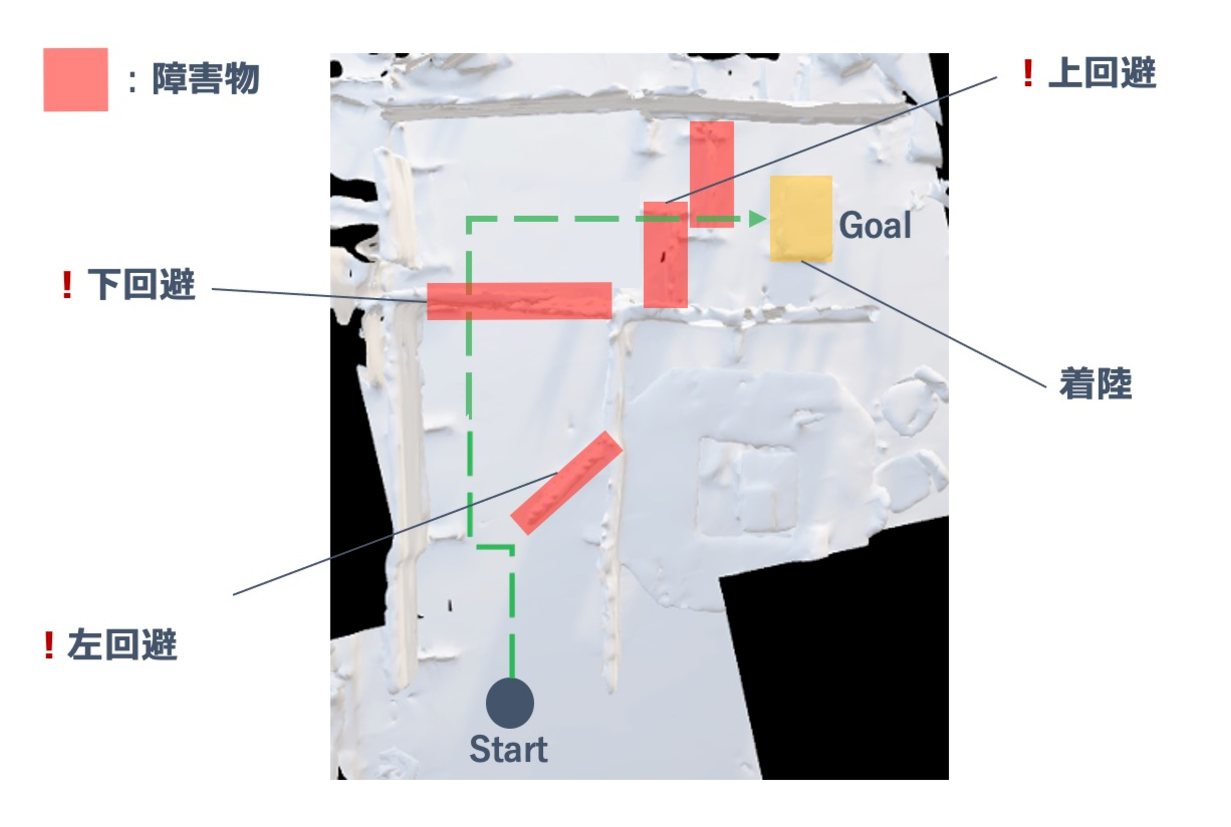
\includegraphics[width=\linewidth]{img/04_experiment.eps}
\caption{実験環境}
\ecaption{Experimental Environment}
\label{fig:04_experiment}
\end{figure}


% -----------------------------------------------------------------




% --------------------------- Figure  ---------------------------

% \begin{figure}[b]
% 	\caption{アンケート項目}
% 	\centering
%     \includegraphics[width=\linewidth]{img/likert1.eps}
%     \label{tab:Likert1}
% \end{figure}

% \begin{figure}[b]
% 	\caption{ARのみのアンケート項目}
% 	\centering
%     \includegraphics[width=\linewidth]{img/likert2.eps}
%     \label{tab:Likert2}
% \end{figure}

% -----------------------------------------------------------------

\subsection{評価項目}
提案方式の有効性を評価するにあたり,ドローン技術の熟練度による差を出さないために,Telloの速度,一度に進む距離,旋回角度は事前に設定している.またサーバのスペック,サーバよりTelloへ送信するコマンドのパラメータの設定を表\ref{tab:server_spec},表\ref{tab:command_parameter}に示す.
本研究では,各方式における,操縦者がタスクを完了するまでの操縦時間,障害物への衝突警告回数の2項目による客観的な評価と,参加者へのアンケート,自由回答による主観的な評価を記録した.障害物の衝突警告回数では,実際に衝突してしまう恐れがあるため,操縦者がドローンを進行させようとしている方向に存在する障害物との距離を計測し,距離が0.3 m以内の際に操縦者へ警告がされるようになっている.表\ref{tab:command_parameter}に示すように,ドローンの進行距離を0.3 mとしているため,衝突警告距離の閾値を0.3 mとした.また参加者へのアンケートでは,主観的な認識と好みを測定するために,7ポイントのリッカート尺度のアンケートを実施した.アンケートでは一人称視点方式とARを利用した3つの各方式を比較できるように実施し,また,AR同士での比較が行えるように,ARを用いた方式のみ別途アンケートを実施した.一人称視点方式とARを用いた3つの各方式を比較するアンケートでは,安心な操縦できたか,危険な障害物を判断できたかの2項目を設けた.また,ARを用いた方式のみを比較するアンケートでは,状況把握が容易だったか,自信を持って操縦を行えたかの2項目を設けた.実験の最後には,参加者にはどの方式が最も操縦性が良かったかを選択し,なぜその方式が良かったのか,また,なぜ他の方式を選択しなかったかという項目を設けた.タスク完了までの平均操縦時間には一次元配置分散分析(one-way analysis of variance:以下,ANOVA)を用いて統計解析した.また,Post-hoc検定では,Tukey’s Honestly Significant Difference(Tukey HSD)検定を行い,各方式の比較を行なった.平均衝突警告回数,アンケート結果では,Friedman検定を行い,Post-hoc検定ではBonferroni法を行い,各方式の比較を行なった.


% --------------------------- Figure  ---------------------------

 \begin{table}[tb]
  \caption{サーバのスペック}
  \ecaption{Server Performance}
  \label{tab:server_spec}
  \centering
  \begin{tabular}{ll}
  \noalign{\smallskip}\hline\noalign{\smallskip}
    OS     & macOS 11.0.1       \\
    CPU     & 2.4 GHz Intel Core i4       \\
    メモリ     & 8 GB       \\ 
    使用言語     & Python 2.7       \\
    \noalign{\smallskip}\hline
  \end{tabular}
\end{table}

\begin{table}[tb]
  \caption{ドローンへ送信するコマンドのパラメータ}
  \ecaption{Parameters of the Command to Be Sent to the Drone}
  \label{tab:command_parameter}
  \centering
  \begin{tabular}{ll}
    \hline\noalign{\smallskip}
    命令コマンド &  パラメータ       \\
    \noalign{\smallskip}\hline\noalign{\smallskip}
    前進後退     & 0.3 m       \\
    左右移動     & 0.3 m       \\
    上昇下降     & 0.3 m       \\
    左右旋回     & 20 度       \\
    送信間隔     & 0.3 s       \\
    \noalign{\smallskip}\hline
  \end{tabular}
\end{table}

\begin{figure}[tb]
\centering
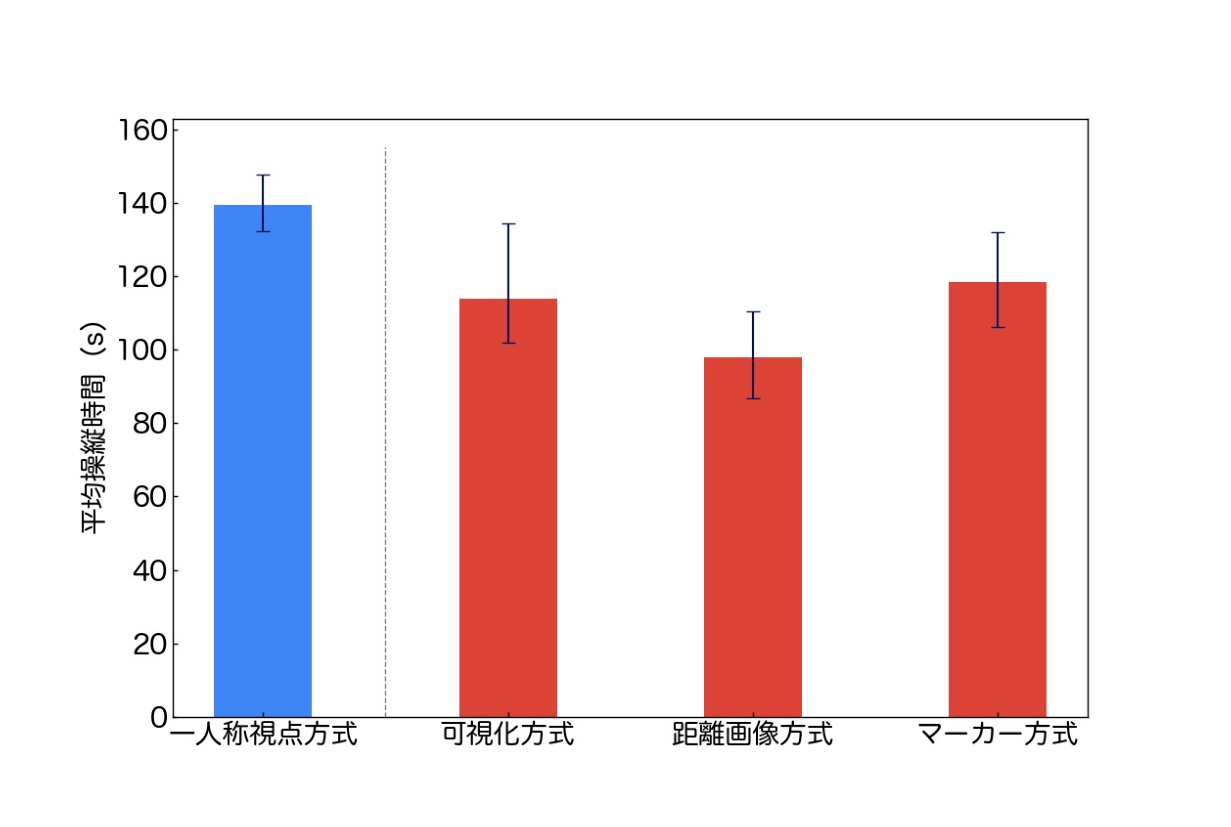
\includegraphics[width=\linewidth]{img/04_bar1.eps}
\caption{平均操縦時間}
\ecaption{Average Maneuvering Time}
\label{fig:04_bar1}
\end{figure}

\begin{figure}[tb]
\centering
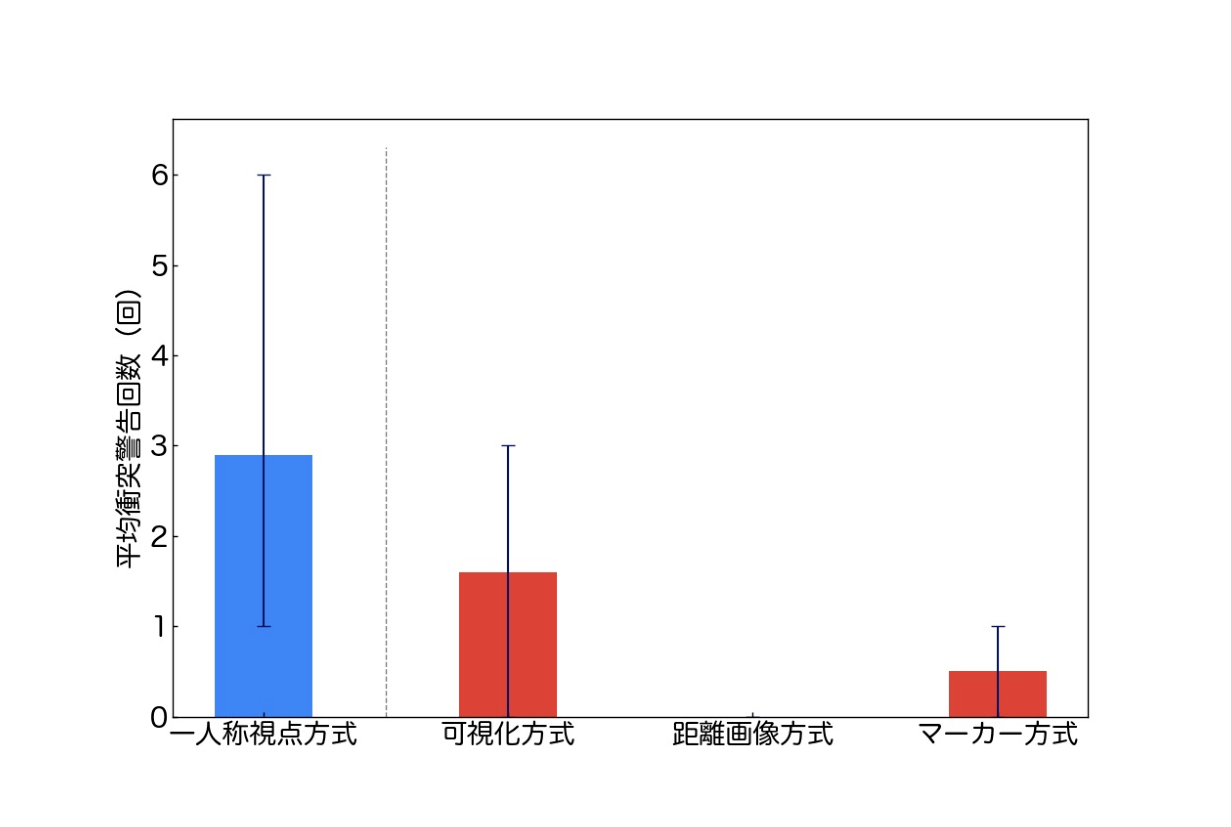
\includegraphics[width=\linewidth]{img/04_bar2.eps}
\caption{平均衝突警告回数}
\ecaption{Average Number of Conflict Warning Returns}
\label{fig:04_bar2}
\end{figure}

% -----------------------------------------------------------------

\subsection{客観的結果}
\label{result_1}
タスクを完了するまでの平均操縦時間の評価結果を図\ref{fig:04_bar1}に示す.
平均操縦時間では,ANOVAで4群間に有意差を示した($F$(3,36) = 48.35, $p = 1.04e-12 $).Tukey HSD検定を用いた多重比較では,一人称視点方式とARを用いた各方式を比較した場合,可視化方式($p < 0.001$),距離画像方式($p < 0.001$),マーカー方式($p < 0.001$)となり,平均操縦時間は有意に減少することがわかった.ARを用いた方式同士では,距離画像方式と各方式を比較した場合,可視化方式($p < 0.001$),マーカー方式($p < 0.001$)となり,有意に操縦時間が減少したことがわかった.しかし,マーカー方式と可視化方式の間では,有意にタスク完了時間が減少しないことが分かった($p = 0.545$).
\par
次に,障害物への平均衝突警告回数の結果を図\ref{fig:04_bar2}に示す.平均衝突警告回数では,Friedman検定の結果,4群間に有意差を示したため($p < 0.05$),Bonferroni法の多重比較($p < 0.05$)を行った.その結果,一人称視点方式とマーカー方式,距離画像方式の間には有意差を示したが,可視化方式との間では有意差は示さなかった($p = 0.163$).また可視化方式は,マーカー方式との間には有意差を示さなかったが($p = 0.069$),距離画像方式との間には有意差を示した.


\subsection{主観的結果}
\label{result_2}
アンケートによる各方式を比較した結果を図\ref{fig:04_likert1},\ref{fig:04_likert2}に示す.
一人称視点方式を含むアンケート結果では,操縦の安心度,危険な障害物知覚の2項目に対してFriedman検定を行ったところ,有意差を示した($p < 0.05$).それぞれの結果に対しBonferroni法の多重比較($p < 0.05$)を行ったところ,操縦の安心度では,一人称視点方式とマーカー方式,距離画像方式間に有意差を示した.また距離画像方式は,可視化方式,マーカー方式との間に有意差を示した.危険な障害物を判断できたかを確認する項目では,一人称視点方式と距離画像方式,マーカー方式の間に有意差を示した.また,距離画像方式は可視化方式,マーカー方式との間にも有意差を示した.
% \par
% ARを用いた方式のみを比較したアンケートである図\ref{tab:AR_situation},図\ref{tab:AR_confidence},図\ref{tab:AR_distance}でも,状況認識,操縦判断の自信度,距離感の3項目全てにFriedman 検定の結果,有意差を示した(p<0.05).それぞれの結果に対しBonferroni法の多重比較(p<0.05)を行ったところ,状況認識では,距離画像方式のみ可視化方式とマーカー方式の間に有意差を示した.操縦判断の自信度でも同じく,距離画像方式のみ可視化方式とマーカー方式の間に有意差を示した.距離感では,可視化方式と距離画像方式,マーカー方式の間に有意差を示した.

% --------------------------- Figure  ---------------------------

% \begin{figure*}[tb]
% \centering
% \includegraphics[width=\linewidth]{img/04_likert.eps}
% \caption{主観的結果}
% \ecaption{Overview of AR System}
% \label{fig:04_likert2}
% \end{figure*}

\begin{figure}[tb]
\centering
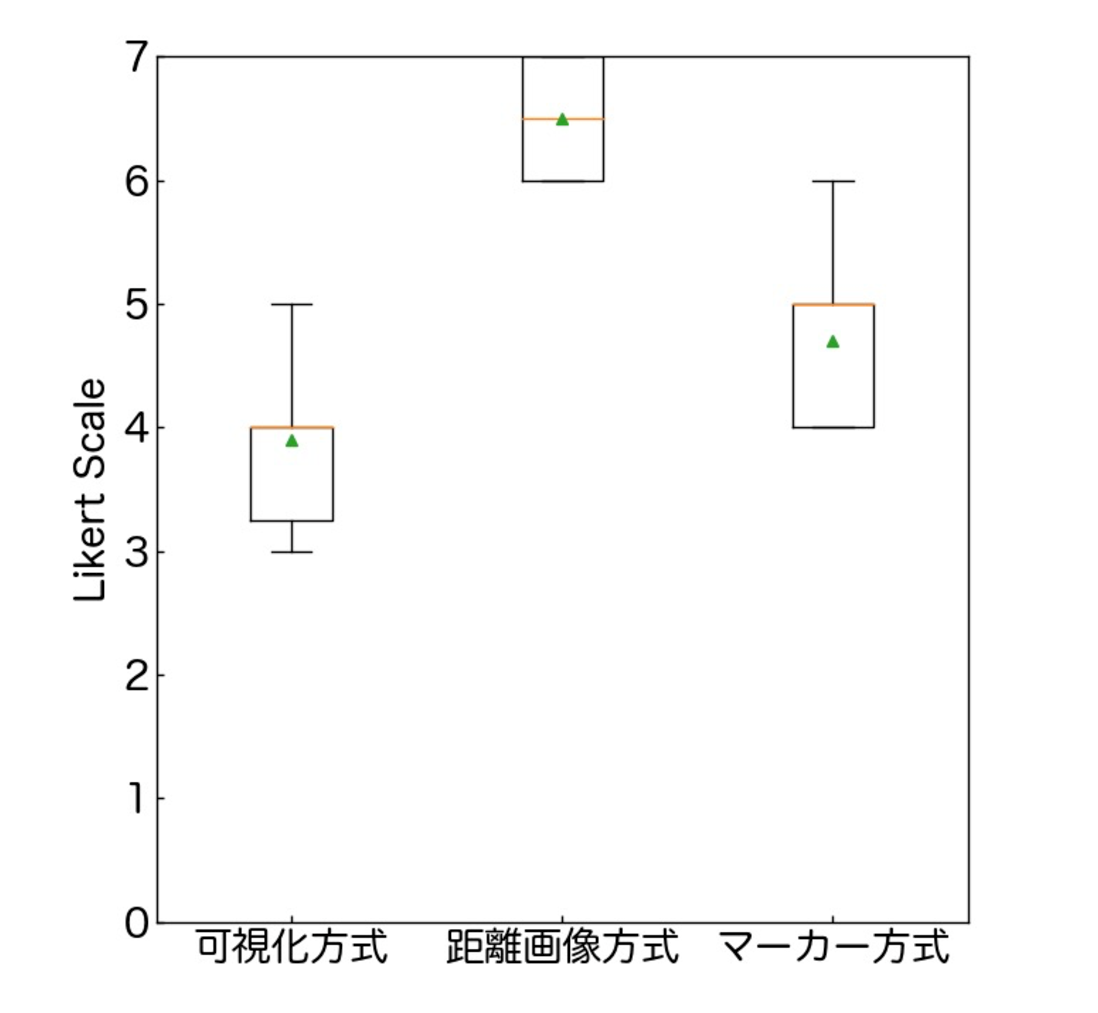
\includegraphics[width=\linewidth]{img/04_likert1.eps}
\caption{操縦の安心度}
\ecaption{Level of Security of Operation}
\label{fig:04_likert1}
\end{figure}

% -----------------------------------------------------------------

% --------------------------- Section5  ---------------------------

\section{考察}
\subsection{AR方式の有用性}
ARを用いた方式では,\ref{result_1}節で述べたように,一貫して一人称視点方式に有意差を示した.
タスク完了までの平均操縦時間では,ARを用いた方式は全て,一人称視点方式と比較して有意に時間が減少している.本研究で想定しているようなドローンは最大飛行時間が短いことが問題点とされている中で,距離画像方式では,従来の操縦法である一人称視点方式の操縦時間と比較して約30\% 減少しているため,作業効率の向上が見込める.また一人称視点方式は,タスク完了までの平均操縦時間と,平均衝突警告回数より,1分間の間だけで約1.25回も衝突の可能性があり,実際の狭小空間における操縦法として危険性が高いことを確認した.
\par
平均衝突警告回数では,ARを用いた方式の中でも,可視化方式は一人称視点方式との間に有意差を示さなかった.そのため,ARを用いた死角領域内の可視化による,三人称視点操縦を実現するだけでは,狭小空間での操縦が未だ危険なことを示した.しかし,距離画像方式やマーカー方式のような障害物を知覚するための方式では,一人称視点方式との間において,平均操縦時間,平均衝突警告回数共に有意差を示していた.そのため,ARを用いた死角領域内の可視化だけでなく,ドローン周辺の障害物に対する視覚的支援を行う本提案方式では,ドローン操縦性向上を示せることがわかった.

% --------------------------- Figure  ---------------------------

% \begin{figure*}[tb]
% \centering
% \includegraphics[width=\linewidth]{img/04_likert.eps}
% \caption{主観的結果}
% \ecaption{Overview of AR System}
% \label{fig:04_likert2}
% \end{figure*}

\begin{figure}[tb]
\centering
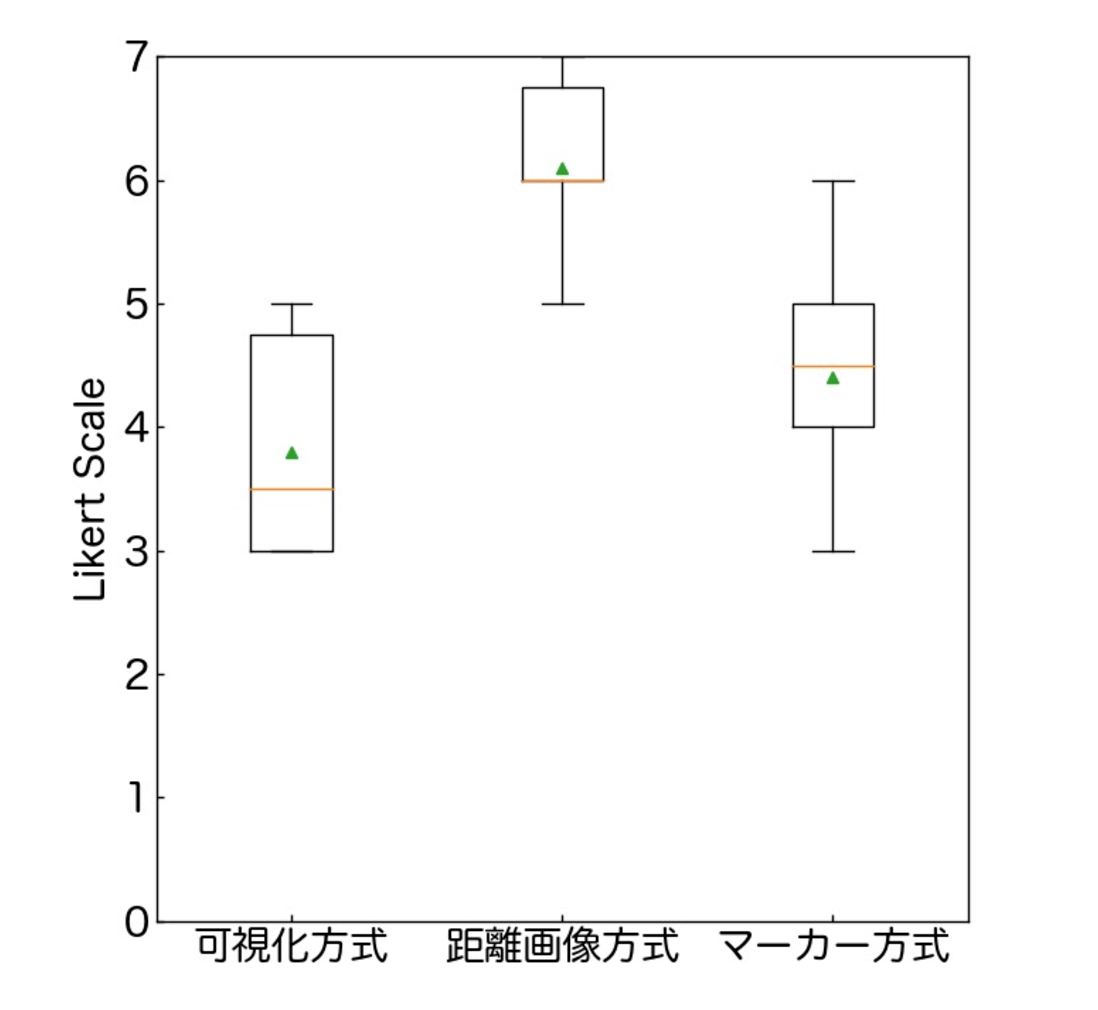
\includegraphics[width=\linewidth]{img/04_likert2.eps}
\caption{危険な障害物知覚}
\ecaption{Dangerous Obstacle Perception}
\label{fig:04_likert2}
\end{figure}
% -----------------------------------------------------------------
\subsection{AR方式の比較の考察}
\subsubsection{客観的結果}
\ref{result_1}節で述べた,客観的結果におけるAR方式同士の有意差について考察する.
タスク完了までの操縦時間では,可視化方式とマーカー方式の間で有意差を示さなかった.
実験参加者の自由回答では,マーカー方式では,操縦の際に躊躇ってしまう傾向があり,また,
可視化方式では,操縦の際に思い切って進む傾向があった.

このことから,マーカー方式では1箇所のみ危険な場所に目印を付けているため,操縦に躊躇いが生じ,慎重になる一方で,可視化方式では,どこの障害物が危険か判断できないため,思い切って操縦するため,マーカー方式では可視化方式と比べ,操縦時間が長くなっていると推測される.
また衝突警告回数では,距離画像方式とマーカー方式の間では有意差を示さなかった.しかし,実際にドローン操縦を行う際にドローンの衝突は0に収めなければならないことを考えると,距離画像方式では衝突警告回数を0回に収めたことより,有意な結果であると推測される.

\subsubsection{主観的結果における考察}
\ref{result_2}節で述べた,主観的結果におけるAR方式同士の有意差について考察する.
アンケート結果では,可視化方式とマーカー方式の間において,一貫して有意差を示さなかった.
実験参加者の自由回答では,マーカー方式では,気になる障害物に対して目印を示さない傾向があった.
このことから,ドローン周辺に衝突の可能性のある障害物が2つ以上ある際に,操縦者が手に入れたい障害物までの距離感を示さない可能性があるため,可視化方式と比べ有意差を示さなかった.

\subsection{全体の考察}
実験の最後にどの方式が最も効果的であったかを選択してもらった結果,9名が距離画像方式を選択し,1名がマーカー方式を選択した.距離画像方式を選択した理由として,障害物までの距離を色で示していることによって距離感を掴みやすかった点や,見える景色全体に色がついているため,どの範囲まで動かすことができるかが分かりやすかった点が挙げられた.一方で,他の方式を選択しなかった理由として,一人称視点方式では,上下の障害物までの距離感が掴づらかった点や,周囲の確認に不安があった点が挙げられた.可視化方式では,全体像は掴めたが状況認識が難しかった点や,距離感に自信を持てない点が挙げられ,マーカー方式では,一方向でしか距離感が分からなかった点や,距離画像方式が全体像が理解が容易だった点が挙げられた.一方でマーカー方式を選択した参加者は,最も近傍の障害物を示してくれる安心感がある点からマーカー方式を選択し,距離画像方式では周囲が赤色になった際に困惑した点や,見えている情報が簡潔でない点から選択しなかった.
以上のことから,狭小空間での操縦では障害物知覚が必要であり,操縦者にとって重要な情報は,最も危ない位置を示すような直感的な情報ではなく,常に周囲の危険性を示す全体的な把握を促せる情報であることがわかった.距離画像方式では,図\ref{fig:04_bar1},\ref{fig:04_bar2}に示すように,他の方式と比べ平均操縦時間の減少,衝突回数の減少を可能にすることができたため,狭小空間による死角領域内の環境下において,ドローン操縦性向上に有効であることを確認した.



% --------------------------- Section6  ---------------------------

\section{おわりに}

小型ドローンは機体の大きさを活かして,インフラ点検や災害調査のような,人間が立ち入れない狭小空間での活躍が増えている.しかし,狭小空間でのドローン飛行では,遮蔽物による視点が遮られる死角領域内での操縦を必要とする.また,従来の操縦法では状況認識が不十分であるため,ドローン周辺に位置する障害物が多い狭小空間では,ドローン操縦は困難である.\par
遮蔽物,障害物が多い狭小空間では,死角領域内におけるドローン飛行の危険性を軽減する必要がある.
そこで本研究では,ARにより操縦者の死角領域内に存在するドローンと周辺環境を可視化し,ドローン周辺の障害物を知覚するためのAR方式を提案する.
本提案方式について,死角領域内でのドローン操縦性を評価実験した.
結果として,ARを利用した方式では実験環境での操縦時間が短く,衝突回数も少なかったことから,狭小空間による死角領域内のドローン操縦性向上を示した.
また,障害物を知覚するためのAR方式では,ドローン周辺の障害物に対し,危険度を色で振り分けている方式が操縦者へ安心を与え,操縦性を向上させたことを示した.




\begin{thebibliography}{10}

\bibitem{Nonami}
野波健蔵:ドローン技術の現状と課題およびビジネス最前,情報管理,Vol.59,No.11,pp.755-763(2017).


\bibitem{Green}
Green S. A. , Chase J. G., Chen X. and Billinghurst M.: Evaluating the Augmented Reality Human-Robot Collaboration System, 
{\it 2008 15th International Conference on Mechatronics and Machine Vision in Practice}, 
pp.521-526(2008).

\bibitem{Zollmann}
Zollmann S., Hoppe C., Langlotz T. and Reitmayr G.:
FlyAR: Augmented Reality Supported Micro Aerial Vehicle Navigation, In 
{\it IEEE Transactions on Visualization and Computer Graphics}, 
vol.20, no.4, pp.560-568(2014). 


\bibitem{syohou}
東京消防庁:屋内空間におけるドローンの活用に関する検証,
\urlj{https://www.tfd.metro.tokyo.lg.jp/hp-gijyutuka/shyohou2/56/56-3.pdf}

\bibitem{Walker}
Walker M., Hedayati H., Lee J. and Szafir D.: Communicating Robot Motion Intent with Augmented Reality, 
{\it HRI '18: Proceedings of the 2018 ACM/IEEE International Conference on Human-Robot Interaction}, 
pp.316-324(2018).

\bibitem{Hedayati}
Hedayati H., Walker M. and Szafir D.: Improving Collocated Robot Teleoperation with Augmented Reality, In 
{\it Proc. ACM/IEEE International Conference on Human-Robot Interaction (HRI '18)}, 
pp.78-86(2018).

\bibitem{Kameda}
Kameda Y., Takemasa T., and Ohta Y.: Outdoor see-through vision utilizing surveillance cameras, 
{\it Third IEEE and ACM International Symposium on Mixed and Augmented Reality}, 
pp.
151-160(2004).

\bibitem{Liu}
Liu C. and Shen S.: An Augmented Reality Interaction Interface for Autonomous Drone, 
{\it IEEE/RSJ International Conference on Intelligent Robots and Systems (IROS)}, 
pp.11419-11424(2020).

\bibitem{Erat}
Erat O., Isop W. A., Kalkofen D. and Schmalstieg D.: Drone-Augmented Human Vision: Exocentric Control for Drones Exploring Hidden Areas, In 
{\it IEEE Transactions on Visualization and Computer Graphics}, 
vol.24, no.4, pp.1437-1446(2018).

\bibitem{Yamada}
山田開斗, 薄羽大樹, 宮下芳明:ドローン操縦におけるクロッシング評価, 研究報告ヒューマンコンピュータインタラクション(HCI), issue.2, no.2, pp.1-6(2019).

\end{thebibliography}
\end{document}
